\chapter{Tu primer vuelo, paso a paso}
\label{cap:primer-vuelo}

\begin{enpocas}
Lanzar una misión completa, saber qué mirar en cada ventana, leer el resultado y cambiar una cosa a la
vez.
\end{enpocas}

\section{Antes de empezar}

\begin{itemize}
  \item La instalación del capítulo~\ref{cap:instalacion} ya está hecha y compilada (\cod{colcon build}).
  \item No hay otra simulación de PX4 abierta (comparten el puerto 8888).
  \item Si la campaña está corriendo, espera a que termine o usa otra partición y otro dominio
        (capítulo~\ref{cap:pilotos}).
\end{itemize}

\section{Paso 1: lanzar}

\begin{lstlisting}[style=bash]
source ~/ros2_ws/install/setup.bash
ros2 launch mision simulacion.launch.py
\end{lstlisting}
En unos 30~segundos aparecen Gazebo con el bosque, la terminal y la consola de MAVProxy, y el mapa.
El Tarot 650 despega del origen. La terminal de ROS va diciendo lo que pasa (esta salida es de una
corrida del 23 de octubre, con el x500; con el Tarot los mensajes son los mismos):
\begin{lstlisting}
[mision]: misión fija con controlador cascada: 8 puntos de ruta a 30.0 m
[mision]: despegue -> barrido
PERSONA 1 LOCALIZADA 2026-10-23 08:28:21
  GPS: 19.482273, -99.244990  (19°28'56.2"N 99°14'42.0"W)
[mision]: barrido -> aterrizaje
[mision]: 1/1 personas localizadas, 14 falsas alarmas, error 0.43
[mision]: misión terminada en 237 s; RMSE de seguimiento 0.07 m; registro en ...
\end{lstlisting}

\section{Paso 2: mirar}

\begin{description}
  \item[Gazebo:] el dron, el bosque y, a la derecha, el panel ``Detección de personas'' con la
        imagen de la cámara y los recuadros de YOLO.
  \item[Mapa de MAVProxy:] la ruta en franjas, la trayectoria recorrida y cada persona avisada.
  \item[Terminal:] los avisos con GPS y enlace a Google Maps.
\end{description}

\begin{figure}[H]
\centering
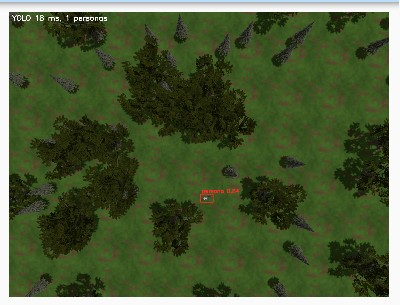
\includegraphics[width=0.85\textwidth]{panel_yolo_personas.jpg}
\caption{El panel de detección durante el barrido.}
\end{figure}

\section{Paso 3: leer el resultado}

\begin{lstlisting}[style=bash]
python3 -c "import json; r=json.load(open('$HOME/resultados/corrida.json')); \
print(r['personas_localizadas'], '/', r['personas'], r['falsas_alarmas'], r['duracion_s'])"
\end{lstlisting}
El significado de cada campo está en la tabla de métricas del capítulo~\ref{cap:mision}.

\section{Paso 4: cambiar una cosa}

\begin{lstlisting}[style=bash]
ros2 launch mision simulacion.launch.py estrategia:=reobs             # con re-observación
ros2 launch mision simulacion.launch.py oclusion:=alta semilla:=4     # bosque denso
ros2 launch mision simulacion.launch.py controlador:=red              # vuela la red neuronal
ros2 launch mision simulacion.launch.py piloto:=ardupilot             # con ArduPilot
ros2 launch mision simulacion.launch.py vehiculo:=x500                # con el x500 de PX4
ros2 launch mision simulacion.launch.py gui:=false salida:=$HOME/r.json   # sin ventanas
\end{lstlisting}

\begin{ejercicio}
Vuela la semilla 1 en oclusión alta con \cod{estrategia:=fija} y luego con \cod{reobs}. ¿Cuántas
personas encontró cada una, y cuánto tardó? Luego repite con la semilla 2. ¿Se mantiene la conclusión?
\end{ejercicio}

\begin{ejercicio}
Vuela con \cod{latencia_extra_ms:=300}. ¿Cuánto crece el error de localización? ¿Por qué? (Pista: a
3~m/s, 300~ms son 0.9~m.)
\end{ejercicio}

\section{Si algo falla}

\begin{longtable}{>{\raggedright\arraybackslash}p{5cm}p{10cm}}
\toprule
\textbf{Síntoma} & \textbf{Causa y remedio} \\ \midrule \endhead
El dron no despega & PX4 no recibe la odometría o el agente no arrancó: revisa que no haya otra
simulación en el puerto 8888 (\cod{pgrep -a MicroXRCE}). \\
La memoria se llena en minutos & Gazebo cargó \cod{GstCameraSystem}; el \emph{launch} lo evita, no
uses \cod{make px4_sitl gz_...} para estas misiones. \\
Ninguna persona encontrada & ¿El detector cargó los pesos? Busca \cod{[detector]} en la terminal y
mira \cod{/detecciones}. \\
Quedan ventanas abiertas & \cod{pkill -f mavproxy}; el \emph{launch} normalmente las cierra. \\
Con \cod{vehiculo:=x500} y \cod{controlador:=red} PX4 vuela mal & PX4 lleva compilada la red del Tarot;
reinstala la del x500 con \cod{instalar_px4.sh} (capítulo~\ref{cap:tarot650}). \\
\bottomrule
\end{longtable}
